\section{timer.c File Reference}
\label{timer_8c}\index{timer.c@{timer.c}}
{\tt \#include $<$msp430x16x.h$>$}\par
{\tt \#include $<$stdio.h$>$}\par
{\tt \#include $<$stdlib.h$>$}\par
{\tt \#include $<$signal.h$>$}\par
{\tt \#include \char`\"{}ueaclib.h\char`\"{}}\par
{\tt \#include \char`\"{}ueac.h\char`\"{}}\par
{\tt \#include \char`\"{}conversion.h\char`\"{}}\par
{\tt \#include \char`\"{}filter.h\char`\"{}}\par
{\tt \#include \char`\"{}global.h\char`\"{}}\par
{\tt \#include \char`\"{}lla.h\char`\"{}}\par


Include dependency graph for timer.c:\begin{figure}[H]
\begin{center}
\leavevmode
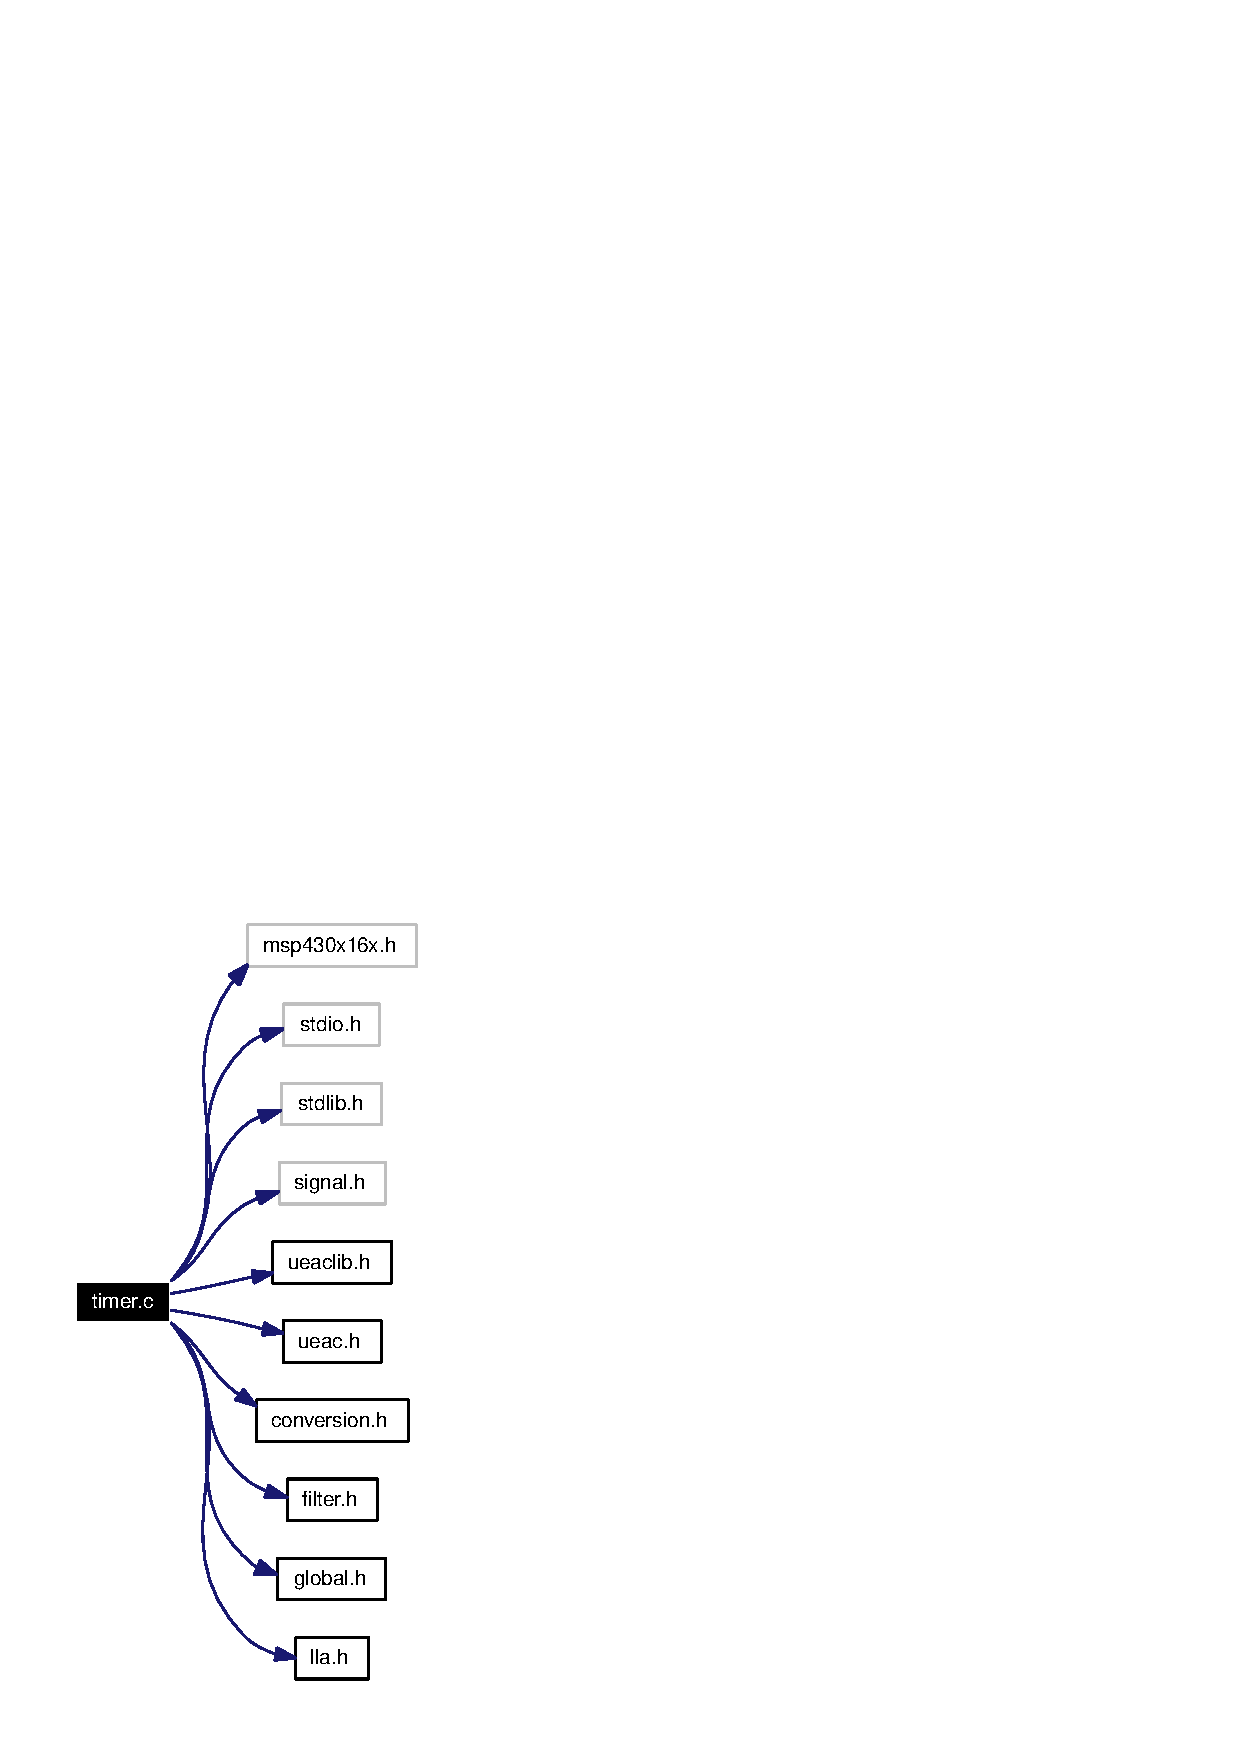
\includegraphics[width=100pt]{timer_8c__incl}
\end{center}
\end{figure}
\subsection*{Functions}
\begin{CompactItemize}
\item 
{\bf timer\_\-a0\_\-irq} ()
\item 
void {\bf delay\_\-1\_\-25m\-S} (int count)
\end{CompactItemize}


\subsection{Function Documentation}
\index{timer.c@{timer.c}!delay_1_25mS@{delay\_\-1\_\-25mS}}
\index{delay_1_25mS@{delay\_\-1\_\-25mS}!timer.c@{timer.c}}
\subsubsection{\setlength{\rightskip}{0pt plus 5cm}void delay\_\-1\_\-25m\-S (int {\em count})}\label{timer_8c_a1}




Definition at line 116 of file timer.c.

References timer\_\-tick.

Referenced by current\_\-output\_\-calibration(), main(), print\_\-grid\_\-i(), scan\_\-leds(), and scan\_\-probes().

\footnotesize\begin{verbatim}116                              {
117   int tick_counter=0;
118   while (tick_counter<count) {
119     if (timer_tick) {
120       tick_counter++;
121       timer_tick=0;
122     }
123   }
124 }
\end{verbatim}\normalsize 


\index{timer.c@{timer.c}!timer_a0_irq@{timer\_\-a0\_\-irq}}
\index{timer_a0_irq@{timer\_\-a0\_\-irq}!timer.c@{timer.c}}
\subsubsection{\setlength{\rightskip}{0pt plus 5cm}timer\_\-a0\_\-irq ()}\label{timer_8c_a0}


Timer A1 Interupt Handler

Timer A is used as the time base for the scheduler. This interrupt occurs every 1.25m\-S.

Definition at line 66 of file timer.c.

References evaluate\_\-lla(), high\_\-time\_\-limit, led\_\-pwm(), led\_\-screen\_\-enable, lla\_\-input\_\-check(), pin\_\-data, start\_\-a2d\_\-converter(), timer\_\-tick, ueac\_\-state, update\_\-a2d\_\-data(), and write\_\-analog\_\-mux().

\footnotesize\begin{verbatim}66                {
67   static int chan_last=0;
68   static int chan_next=0;
69   static char state=0;
70 
71   TACCR0+=0x900;               // Increment the compare register for 2305 ticks into future (625uS)
72   if (!state) {                // evaluate the system every 1.25mS 
73     chan_last=chan_next&0x07;
74     write_analog_mux(++chan_next);
75 
76     update_a2d_data(&pin_data[chan_last],ADC12MEM0);
77     update_a2d_data(&pin_data[8+chan_last],ADC12MEM1);
78     update_a2d_data(&pin_data[16+chan_last],ADC12MEM2);
79     if (chan_last==0) {
80       update_a2d_data(&pin_data[24],ADC12MEM3);
81     }
82 
83     if (lla_input_check(chan_last,&ueac_state)) {
84       high_time_limit[chan_last]=1;
85     }
86     else {
87       high_time_limit[chan_last]=ADC12MEM0>>8;
88     }
89     if (lla_input_check(8+chan_last,&ueac_state)) {
90       high_time_limit[8+chan_last]=1;
91     }
92     else {
93       high_time_limit[8+chan_last]=ADC12MEM1>>8;
94     }
95     if (lla_input_check(16+chan_last,&ueac_state)) {
96       high_time_limit[16+chan_last]=1;
97     }
98     else {
99       high_time_limit[16+chan_last]=ADC12MEM2>>8;
100     }
101 
102     if (lla_input_check(24,&ueac_state)) {
103       high_time_limit[24]=2;
104     }
105     else {
106       high_time_limit[24]=(ADC12MEM3>>8)+1;
107     }
108     evaluate_lla(&ueac_state);
109     start_a2d_converter();
110     timer_tick=1;
111   }
112   state^=1;
113   led_pwm(led_screen_enable);
114 }
\end{verbatim}\normalsize 




Here is the call graph for this function:\begin{figure}[H]
\begin{center}
\leavevmode
\includegraphics[width=288pt]{timer_8c_a0_cgraph}
\end{center}
\end{figure}
